%Her formidles projektets resultater fra testen i kort, nøgtern form, f. eks. ved anvendelse aftabeller, grafer og/eller billeder. De opnåede resultater er dokumenteret detaljeret i projektets bilag, så der kan henvises til dette dokument. Det er vigtigt, at præsentationen af resultaterne er utvetydig, nøgtern og objektiv
\chapter{Results}
This section presents the results of the acceptance test, and a more detailed write-up can be found in section 8 of the Documentation. Table \ref{table:acceptance_test_results} shows the overall results of the acceptance tests.

Use cases 1-4 deal with the creation, deletion, editing, and activition of user profiles in the user interface, both main scenarios and an extension. The verification of the Edit parameters menu rested on the result of these tests. New profiles were created as detailed in the test specification, and the deletion function worked as described, even in the edge cases where an active profile was deleted, or the last profile in the list was deleted. Editing and activation worked as described as well, and thus all four tests passed. 

Use case 5 have to do with the diagnostics window of the user interface, and whether data is available for the motors, GPS receiver, and connectivity, as well as a map showing the location and orientation of the boat. This use case passed as well, since all relevant data was updated at the expected interval in the expected format.

Use cases 6-9 cover the functionality of the point to point interface. The system must be able to set markers either by clicking on the map, or setting a latitude/longitude pair, which creates a marker in the specified position. It must also calculate, start traversing, and stop a point to point path. All these four use cases passed the tests.

Finally, use cases 10-13 describe the coverage rectangle interface. Like the previous four, coordinates must be put onto the map by clicking or typing them in, and a path must then be calculated, traversed, and stopped. All four of these use cases have strong similarity to the point to point use cases, and it was thus expected that the result would be the same for these similar tests. This assumption turned out to be true, and all four tests passed in a similar manner to the point to point tests.

The finished hardware and an image of the finished user interface can be seen in figure~\ref{fig:result}.

\begin{figure}[H]
	\centering
	\subfloat[The finished website, opened on the coverage page] {
		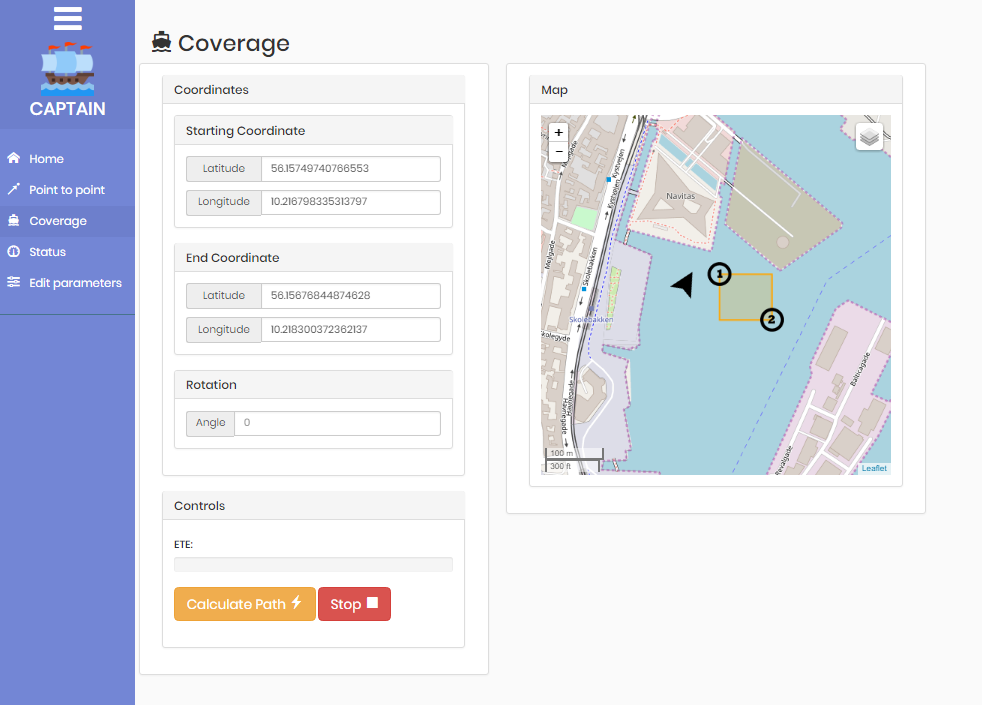
\includegraphics[width=0.45\textwidth]{../Appendix/Project/Dokumentation/Images/Implementation/coverage_page}
		\label{fig:finised_website}
	}
	\hfill
	\subfloat[All hardware put together]{
		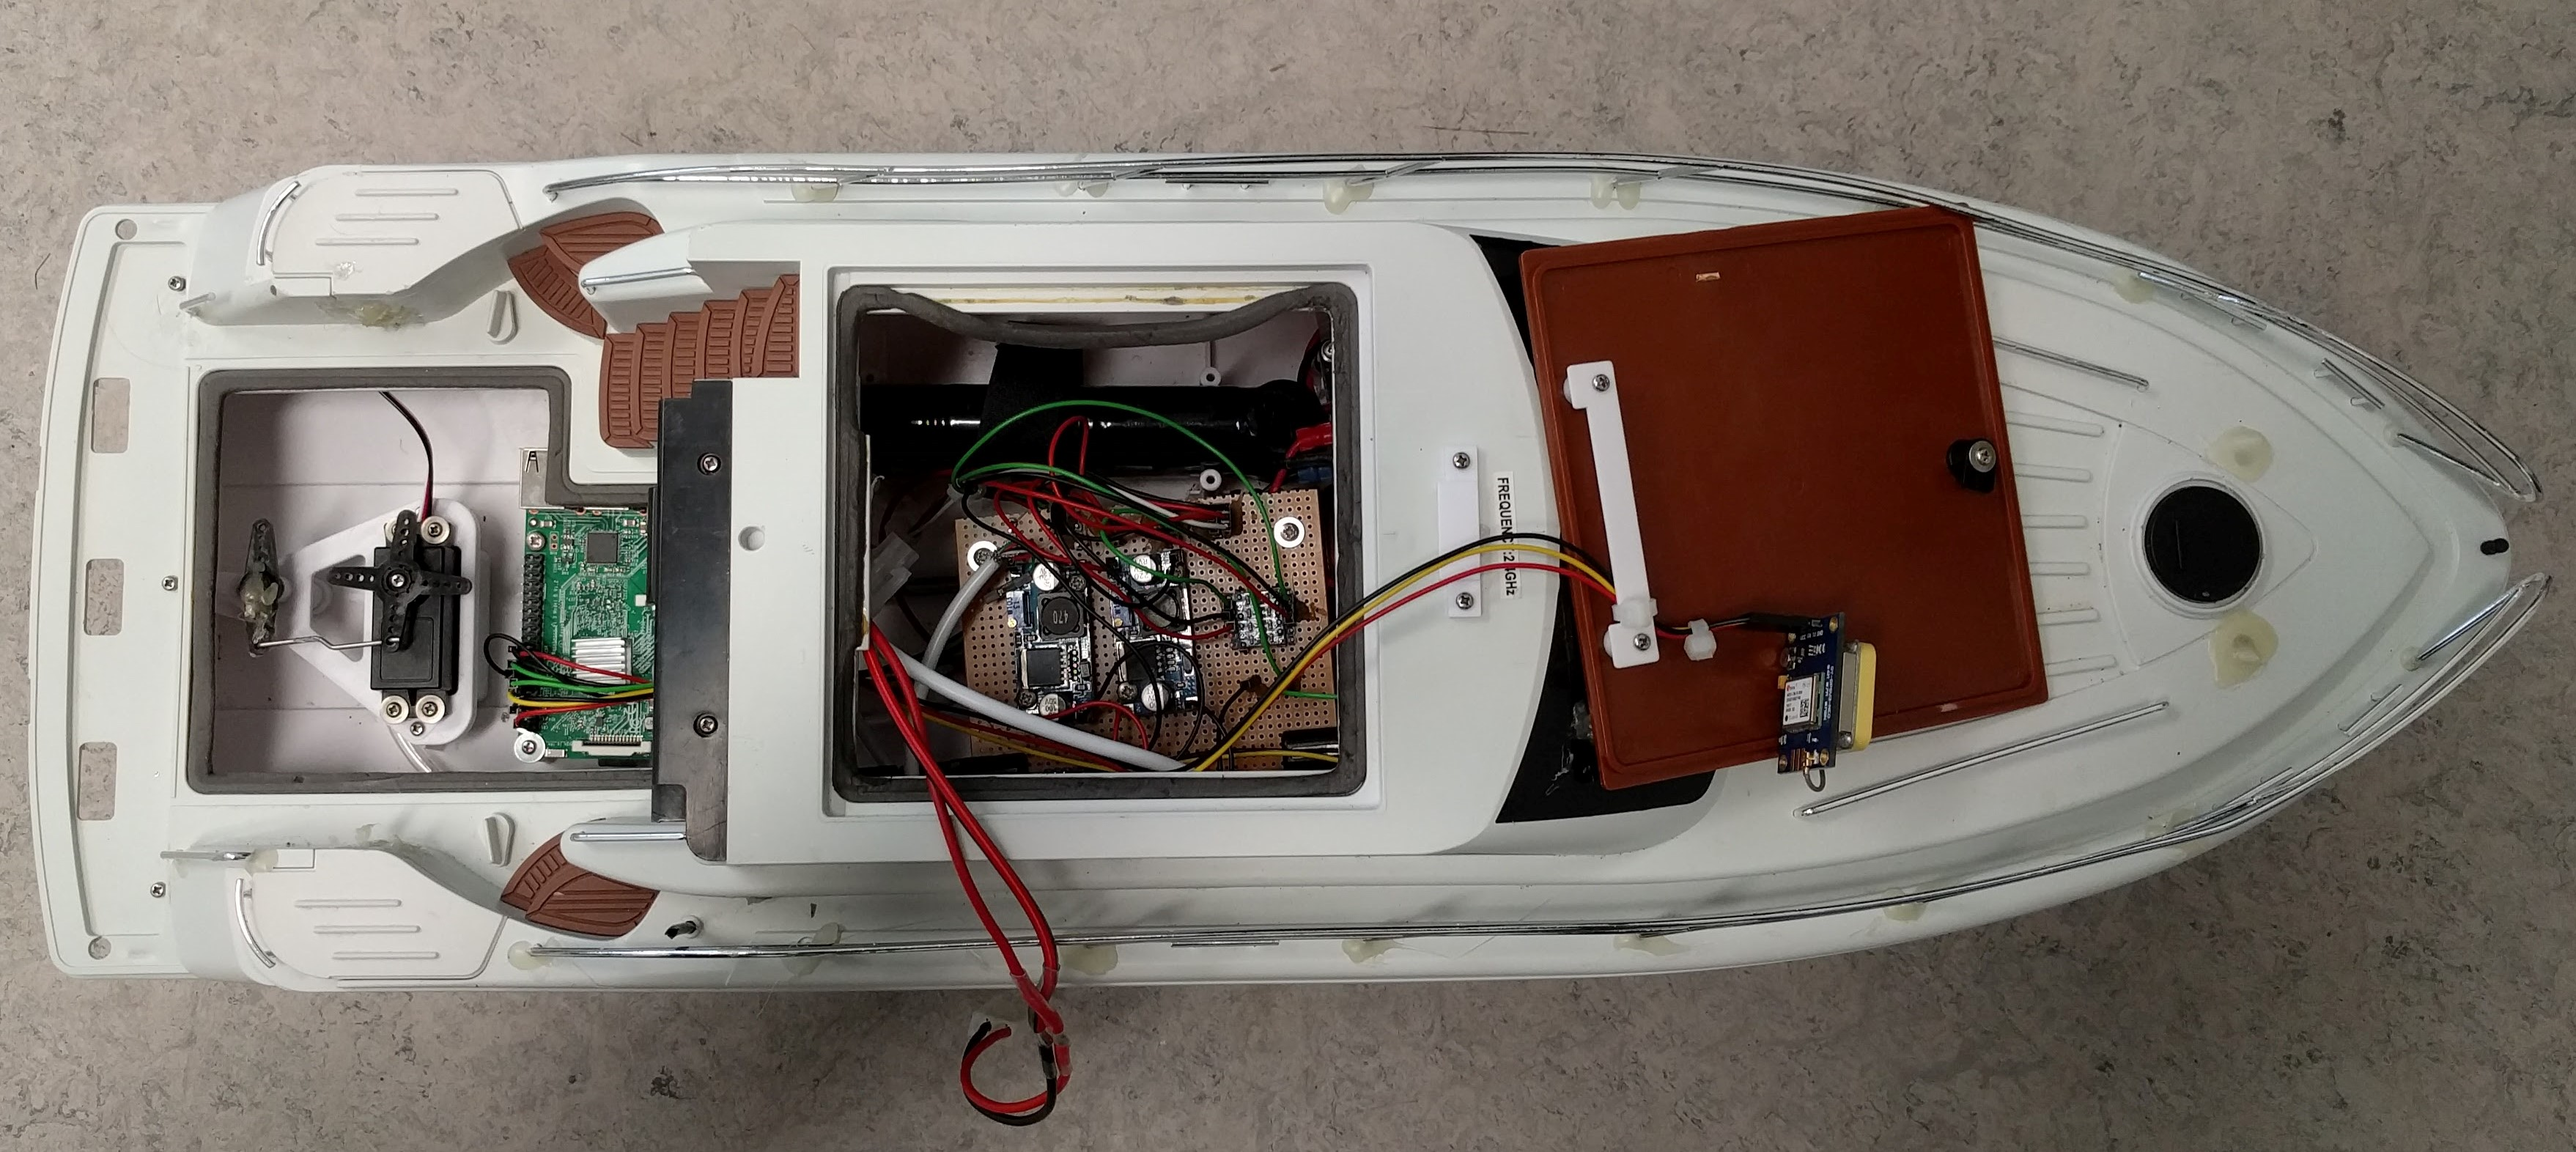
\includegraphics[width=0.45\textwidth]{../Appendix/Project/Dokumentation/Images/Implementation/all_hardware_in_boat}
		\label{fig:finished_boat_hardware}
	}
	\caption{The final product}
	\label{fig:result}
\end{figure}



\begin{table}[H]
\centering
\begin{tabular}{|c|c|}
\hline 
\textbf{Use case} & \textbf{Status}\\ 
\hline 
UC1 - New parameter profile & Passed \\ 
\hline 
UC2 - Delete parameter profile & Passed \\ 
\hline 
UC2 - Delete Parameter profile extension & Passed \\ 
\hline 
UC3 - Edit parameter profile & Passed \\ 
\hline 
UC3 - Edit parameter profile extension & Passed \\ 
\hline 
UC4 - Set active parameter profil & Passed \\ 
\hline 
UC5 - Request diagnostics & Passed \\ 
\hline 
UC6 - Set point to point destination & Passed \\ 
\hline 
UC6 - Set point to point destination alternate flow & Passed \\ 
\hline 
UC7 - Calculate point to point path & Passed \\ 
\hline 
UC8 - Run point to point path & Passed \\ 
\hline 
UC9 - Stop point to point path & Passed \\ 
\hline 
UC10 - Set coverage area & Passed \\ 
\hline 
UC10 - Set coverage area alternate flow & Passed \\ 
\hline 
UC11 - Calculate coverage path & Passed \\ 
\hline 
UC12 - Run coverage path & Passed \\ 
\hline 
UC13 - Stop coverage path & Passed \\ 
\hline 
\end{tabular} 
\caption{Overview of acceptance test results}
\label{table:acceptance_test_results}
\end{table}